%!TEX root = ../../thesis.tex
%!TEX enableSynctex = true
%*******************************************************************************
%****************************** Third Chapter **********************************
%*******************************************************************************
% **************************** Define Graphics Path **************************
\ifpdf
    \graphicspath{{Chapter/tweezers/Figs/Raster/}{Chapter/tweezers/Figs/PDF/}{Chapter/tweezers/Figs/}}
\else
    \graphicspath{{Chapter/tweezers/Figs/Vector/}{Chapter/tweezers/Figs/}}
\fi

\chapter[Light-sheet microscopy combined with remote force measurements]{Light-sheet microscopy combined with remote force measurements}%:\\ \Large Correlating real-time viscoelastic changes with embryonic development}
\epigraph{\textit{The wand chooses the wizard harry}}{--- Olivanderporten}
% Section on what we're trying to achieve
%From Julien:
How multicellular organisms enact the morphogenetic programmes that ensure their characteristic forms remains an enigma.
Genetic screens have yielded an array of essential structural, patterning and signaling pathways with which morphogenesis is orchestrated.
However, morphogenesis is ultimately a physical phenomenon that requires a physical explanation.
In vivo imaging of morphogenesis allows measurements that reveal stereotypical patterns in the cellular behaviour by individual and groups of cells.
These are indicative of active force generation but are insufficient to construct a quantitative explanation of where forces are generated and how forces propagate within and between tissues.
To overcome these limitations, we require a quantitative characterisation of the physical properties of the tissues involved.
Only with this knowledge are we able to understand how forces propagate within tissues to bring about morphogenesis.
Measurements of the properties of individual cells () and for bulk tissues () have revealed both viscoelastic or visco-elasto-plastic solids ().
[Cell autonomous force generation uses actomyosin-based contractile activity. – need to mention intrinsic forces someplace]   Bulk tissue properties can be estimated using atomic force microscopy to investigate a tissue surface.
Alternatively, micropipette aspiration can probe dissociated cells or explants, however deep tissue cannot be assessed directly.
More recently, techniques have been developed to measure tissue stress and viscoelastic properties, utilising laser ablation,  oil droplets, or embedding tissue explants in matrix gel.
Most recently, ferrofluid droplets have shown that local tissue properties, that change regarding the tissue localisation.
We are still in need of methods that can give a repeated real-time readout of physical properties and relate those measurements to the underlying morphogenetic behaviour.
[**What do we say that makes us different to oil droplets?]

We sought a method that can give a non-destructive, quantitative measurement of local tissue physical properties at the length scale of a few cells, completed with seconds to minutes and repeatable over developmentally-significant periods.
We chose to use biologically-compatible paramagnetic beads, implanted into the developing zebrafish embryo
A four-pole electromagnetic device was built that produces a controlled magnetic field gradient in 3D, such that a bead can be moved with known force.
Tracking bead movement gives the dynamic material properties of the surrounding tissue.
In a first test of this approach, we have followed the emergence of the first cohesive tissue of the zebrafish blastula, between the “high” to “sphere” stages of development().
After the mid-blastula transition, mesenchymal blastomeres become first motile and adherent to form the tissue that will go on to contribute to the first morphogenetic movement of the embryo.
We could show for the first time that a three-fold elevation of tissue elasticity and viscosity are associated with this development.
This elevation is dependent upon E-cadherin-based adhesions and Rac-1 dependent cell protrusive activity, abrogating either interfered with these developmental changes.
Interestingly, reducing Rho-kinase dependent cell contractility increased both tissue viscosity and elasticity and raised the number of cell protrusions.
To better comprehend the cellular basis for the physical properties detected by our new method, we combined magnetic tweezers with light sheet microscopy.
Together, this permitted us to correlate a viscoelasticity with cell shape change and a viscosity with cell rearrangements, both cellular changes reduce as tissue elasticity and viscosity increase.
We can now assign the viscoelastic component predominantly to cell shape change and viscosity to cell rearrangement.
[Some of this really belongs in the discussion but will leave here for now]
[If stiffness is explained by cell volume, then effect should be proportional to change in r, r decreases just a few %, while stiffness changes 3x][stress stiffening]
*** how much “plastic” change is rearrangement of extracellular space? ***

\section{Tissue dynamics in developing organisms}
\subsection{Danio Rario}
%From Fran edited
The zebrafish (\emph{Danio rerio}) is a key model organism for vertebrate development.
It shares features of its body plan and developmental stages with Xenopus, the chicken, and the mouse (Wolpert et al, 2007), indicating existence of conserved developmental mechanisms of interest.
These mechanisms rely on organism-wide, reproducible patterns of cellular division, migration, death and differentiation, which occur throughout the organism during development as well as adult life.
As this cellular behaviour arises within the context of organism-wide signalling events, a truly complete understanding of the processes shaping them requires whole-organism imaging.
Of the vertebrate model organisms, the zebrafish is best suited for whole organism imaging from fertilisation until hatching/birth.
The embryo is transparent and small, but can still be physically manipulated, and develops outside the mother allowing for imaging uninhibited by surround tissue from the mother.
Zebrafish grow is rapid, a single cell of a diameter of 0.7 mm becomes a 3.5 mm-long larva within three days %TODO see table
%(see table 1 for overview, Kimmel et al (1995) for detailed description).
Finally, Zebrafish are suitable for genetic studies, the genome is fully sequence and there exist tools for genetic manipulation.
Breeding is simple, sexual maturity occurs at three months post fertilisation making for easy cross-breeding %TODO cite (D'Costa \& Shepherd, 2009)
, and the costs of keeping zebrafish are lower than that of other vertebrates due to their low space requirements and minimal handler time for each. %TODO cite (Lieschke \& Currie, 2007).

%Additionally, the zebrafish is suitable for genetic studies: its genome sequence and tools for genetic manipulation are available, breeding is easy and possible from three months after fertilisation (D'Costa \& Shepherd, 2009), and the costs of keeping zebrafish are low compared with other vertebrates (Lieschke \& Currie, 2007).
%From Fran
%\subsection{Embryonic rheology}
\section{Methods of measuring tissue dynamics}
%\section{Magnetic tweezers combined with Light-sheet microscopy}
%Bit on remote force stuff

The force generation requirements for the investigation of cellular morphogenesis limit greatly which techniques might be suitable for force application and measurement: the forces must be applied in the \SI{10}{\micro\meter}-\SI{100}{\micro\meter} length scale, of a similar length to the size of a cell.
The magnitude of these forces must be in the \SI{100}{\pico\meter} - \SI{100}{\nano\meter} range, of a similar magnitude to the forces that we would expect the cells to be able to generate.
It is also desirable for the process to result in minimal heat and light exposure to the organism, as well as to be minimally invasive.
Immediately, potentially suitable techniques such as mechanical probing, atomic force microscopy, and optical tweezers prove intractable.

Magnetic tweezers operate under the principle of applying a force to a magnetic bead through a magnetic field gradient.
Quite uniquely to this technique is the ability to apply force at a distance.
And so experimental procedures can be designed so that the process is minimally invasive to the organism, which is highly desirable for this particular application.
By choosing a suitable magnetic material for the bead, and designing the electromagnets appropriately, magnetic tweezers are also able to generate the required force range at the required length scales.
Single-pole tweezer systems, where a single electromagnetic solenoid is able to apply a variable force on a bead in one direction, have been used in a number of experiments to understand the dynamics of cellular force responses.
However, to fully characterise the force-generation in cellular rearrangement, it is necessary to generate a magnetic force in an arbitrary direction in three dimensions.

Magnetic tweezers are able to apply a remote force on a magnetic probe through tissue.
Several other techniques exist to probe
%TODO Talk about direct tissue probing using AFM or Optical tweezer

\subsection{Magnetic tweezers}
%% Fix
The design of the magnetic tweezers was based on the previously published design %TODO cite (Vicci 2003)
, which is compatible with large sample like zebrafish embryo and was shown to generate sufficient forces.
This section presents the development of the magnetic tweezers including the imaging chamber required by the LSFM.
%%
The mechanical design of the magnetic tweezers was based on a monopole model.
In this simplification the magnetic field is generated by point sources - monopoles - around a sample containing a magnetic bead.
The sum of the aggregated monopole strengths must equal to zero because, in nature, there are no actual sources or sinks of magnetic flux (i.e. solenoids generate dipole magnetisation).
In this model, a force acting on the bead in the direction of a monopole can be approximated by (Jackson 1962)(Amblard et al. 1996):

The magnetic dipole moment $\mathbf{m}$ induced in the bead by a magnetic field $B$ is given by:

\begin{align}
\textbf{m} = \frac{\pi d^3 }{2 \mu_0} \frac{\mu_r -1}{\mu_r +2}  \mathbf{B}
\intertext{A force, proportional to the magnetic dipole moment, is then exerted on the bead in the presence of magnetic field gradients}
\mathbf{F} = \frac{\pi d^3 }{2 \mu_0} \frac{\mu_r -1}{\mu_r +2}  \mathbf{\nabla} \mathbf{B}^2
\end{align}

where $d$ is the diameter of the bead, $\mu_0$ is the magnetic permeability of free space, $\mu_r$ is the relative magnetic permeability of the bead and $\mathbf{B}$ is the magnitude of the field generated by a magnetic monopole.
B is in the form of Bp/r2 where Bp is the monopole strength and r is the distance from the monopole.
Hence the gradient B of the field is 2Bp/r3 and the force on the bead proportional to 2Bp2/r5  (Vicci 2003).
In the mechanical design of the magnetic tweezers, it was thus desirable to position magnetic poles as close as possible to a sample.

A minimum of four monopoles is required to achieve effective 3D specification of the force acting on the bead.
The optimal configuration is a tetrahedral geometry, where monopoles are distributed on the vertices of a tetrahedron. Deviation from this geometry limits the range and directionality of achievable forces. Finally, only one bead should be used at a time, as agglomeration of beads influences the magnetic field distribution due to the mutual interactions between the beads, and thus disturbs the monopole model (Möller et al. 2003).

The magnitudes and gradients of the magnetic eld in the space between the poles is controlled by four solenoid coils - by varying the currents in these coils independently, we can control the magnitude and direction of the force applied to the bead.

\subsubsection{Model Theory}

The simplest phenomenological model capable to mimic the viscoelastic response of an early development zebra‐fish embryo subject to stress generated by a moving spherical rigid object would be a one‐dimensional linear combination of elastic spring and viscous dash‐pots.
More precisely, the model assumes a parallel spring and dash‐pot (Kelvin‐Voigt model), in series with a second dash‐pot, see Figure %TODO Figure

The model is described by the following parameters: dynamic viscosities $\nu_1$ and $\nu_2$ and elastic stiffness E.
When stress $\sigma$ is applied, the spherical rigid object which in our experiment it is a magnetic bead made of suparparamagnetic nanoparticles embedded into a polyester matrix, moves and its displacement is quantified by strain $\epsilon$.
The same parameter is used to evaluate the recovery phase, i.e. when $\epsilon = 0$.
The experimental protocol we are using consists from two phases: the creep phase where from equilibrium state, at $t=0$ , a constant force is applied instantaneous on the bead and kept for a given time $t_1$ (\SI{60}{\second} ), and the recovery phase where the force is suppressed at $t_1$ and the bead displacement is monitored for sufficient time (\SI{120}{\second}).
To derive model's equations, we recall the viscoelasticity’s fundamental equations. A linear spring is described by:

\begin{align}
  \epsilon &= \frac{1}{E} \label{eq:linearspring}\sigma
  \intertext{while a dash-pot obeys:}
  \dot{\epsilon} &= \frac{1}{\eta}\sigma
  \intertext{The equation for a spring and a dash-pot connected in parallel is:}
  \sigma = \sigma_E + \sigma_{\eta_{2}} &= E \epsilon_p + \eta_{2} \dot{\epsilon_p}\\
  \ln\left(\frac{\sigma}{\eta_{2}}-\frac{E}{\eta_2} \epsilon_p \right) &= -\frac{E}{\eta_{2}}t+\ln C_1
  \intertext{Setting the initial conditions of $\epsilon_p = 0$ at $t = 0$:}
  \epsilon_p &= \frac{\sigma}{E}\left(1-\exp(-\frac{E}{\eta_2}t)\right)
  \intertext{The temporal variation of the dash-pot is ruled by:}
  \sigma = \eta_1 \dot{\epsilon_s} &\implies \epsilon_s = \frac{\sigma}{\eta_1}t
  \intertext{Knowing that $\epsilon = \epsilon_s + \epsilon_p$, The strain variance is therefore:}
  \epsilon &= \frac{\sigma}{\eta_1}t + \frac{\sigma}{E}\left(1-\exp(-\frac{E}{\eta_2}t)\right)
\end{align}

During the second phase that starts at $t_1$, the force is zero $\sigma = 0$ and the total strain is given by the
previous displacement of $\eta_1$ dash‐pot blocked at $t = t_1$ plus the relaxation of Kelvin‐Voigt model.
The later one is described by:

\begin{align}
  E \epsilon_p + \eta_2 \dot{\epsilon_p} = 0 \implies \epsilon_p = C_2 \exp\left(-\frac{E}{\eta_2}t\right)
  \intertext{From the continuity of strain and $t = t_1$, $C_2$ becomes:}
  \frac{\sigma}{\eta_1}t + \frac{\sigma}{E}\left(1-\exp(-\frac{E}{\eta_2}t_1)\right) = C_2 \exp\left(-\frac{E}{\eta_2}t\right)\\
  C_2 = \frac{\sigma}{E}\left(\exp\left( \frac{E}{\eta_2}t_1\right)-1)\right)
  \intertext{So, for $t \geq t_1$ the strain is:}
  \epsilon = \frac{\sigma}{\eta_1}t_1 + \frac{\sigma}{E}\left(\exp\left( \frac{E}{\eta_2}t_1\right)-1)\right)\exp\left(-\frac{E}{\eta_2}t\right)
\intertext{The equations of motion may be summarised as}
  \epsilon =
  \begin{cases}
    \frac{\sigma}{\eta_1}t + \frac{\sigma}{E}\left(1-\exp(-\frac{t}{\tau_2})\right) &\text{for } t\geq t_1\\
    \frac{\sigma}{\eta_1}t_1 + \frac{\sigma}{E}\left(\exp\left( \frac{t_1}{\tau_2}\right)-1)\right)\exp\left(-\frac{t}{\tau_2}  \right) &\text{for } t\leq t_1
  \end{cases} \label{eq:modelfitting}
  \intertext{ where $\tau_2 = \frac{\eta_2}{E}$ } \nonumber
\end{align}

The parameters from eq. (13) need to be reviewed and amended if one intends to link them to experimental data as one applies a known force and looks at the displacement of the bead from its initial position and not to stress and strain.

A bead moving through a viscous fluid could be described by Stokes' law $F = 6 \pi \eta' r \nu$ , where $r$ is the radius of the bead and $\nu$ it's critical velocity. One can rewrite Stokes' law as:

\begin{align}
  F &= 6 \pi \eta' r \frac{dx}{dt} \\
  \implies \frac{F}{\pi r^2} &= 6 \eta' \frac{d}{dt}\frac{x}{r} \\
  \implies \sigma &= 6 \eta' \frac{\epsilon}{dt}
  \intertext{The equation of a dash-pot $\dot{\epsilon} = \frac{\sigma}{\eta}$}
\end{align}

To model the elastic spring, we approximate the elastic response of the tissue due to the bead
displacement, to the Thomson's solution of a point force in an infinite isotropic medium \cite{landau & Lifshitz, Theory of Elasticity}.

The displacement $\mathbf{u}$ in cylindrical coordinates $(p,z)$ for a point force $F_z$ located at the origin and
directed along $z$ axis is given by:

\begin{align}
  \mathbf{u} = \frac{F_z}{4 \pi \mu r }\left[ \frac{pz}{4(1-v)r^2} \hat{p}+\left(1- \frac{p^2}{4(1-v)r^2}\right)\hat{z}\right]\label{eq:thomsons}
\end{align}

Where $\hat{p}$ and $\hat{z}$  are unit vectors, $\mu$ is the shear modulus (deformation at constant volume) and $\nu$ is Poisson's ratio (negative ratio of transverse to axial strain of a specimen under an axial force).
As only forces in the $\hat{z}$ direction are being considering, Equation \eqref{eq:thomsons} becomes:

\begin{align}
  u_z = \frac{F_z}{4 \pi \mu r }\left[\left(1- \frac{p^2}{4(1-v)r^2}\right)\right]
  \intertext{Moreover, if one evaluates the displacement only on $z$ axis where $p=0$, this reduces to:}
  \nabla z =  \frac{F_z}{4\pi \mu r}
  \intertext{In the close proximity of the bead of radius $r_{bead}$ , the displacement is given by:}
  \frac{\nabla z}{r_{bead}} =  \frac{1}{4 \mu} \frac{F_z}{\pi r_{bead}^2} \implies \epsilon = \frac{1}{4\mu} \sigma
  \intertext{Which is equivalent to \eqref{eq:linearspring} when substituting $E$ with $4\mu$ }
\end{align}

\subsection{Magnetic tweezer design}

A square loop of iron was used carry magnetic flux from four solenoids to four embedded magnetic tips.
The lower magnetic tips were mounted at \SI{30}{\degree} azimuthally, this allowed for the very large 1.1 NA LWD objective to image the centre of the magnetic poles.
This orientation of tweezer poles does however leave the design without 10\% of the maximum magnetic field strength that a \SI{45}{\degree} pole mounting would provide (\SI{2.33}{\tesla} ).

%\subsubsection{Mechanics}
% Fitting objectives in
% Keeping fish alive
%\subsubsection{Simulations}
\subsubsection{Imaging Chamber Design}

The image chamber presented was 3D printed to allow for modular and rapid re-design.
Acrylic panels were used to allow for a positioning camera (PiCam) to be placed below the tweezer system.
This aided with the position of the Zebrafish.
The chamber was water tight and featured built-in heating pads to maintain the embryo medium at a comfortable $27^oC$ for the Zebrafish being imaged.

%Contraints specifications and requirements
\subsubsection{Force calibration}

Coordinate systems of the Magnetic tweezers and the light-sheet system needed to be mapped due to the non-linear nature of force of the magnetic field.
This was achieved by defining a origin within the tweezer system itself, where force in every direction was maximal.
This point was then recorded by carefully inserting a fiducial magnetic bead attached to an arm positioned using micrometer screws.
Once the Tweezer system was then fixed to the light-sheet system, the automated stage was carefully driven such that the fiducial bead was at the image centre of the camera and the axial centre of the Piezo stage.
Tweezer positioing was achieved by eye for coarse correction, and then using bright-field image built into the Tweezer chamber to finely position the fiducial bead.

%TODO move this somewhere
3D magnetic field gradient is shaped by a combination of currents to obtain forces of range of 8 nN. Force calibration is realised by analysing the velocities of a 41.17 µm diameter paramagnetic bead in known viscosity silicon oil (characteristics and REF), at different combination of intensity of currents.

\subsubsection{Synchronisation}
The magnetic tweezers were calibrated and automated using a small raspberry pi such that simple RS232 commands could control the amount of force, direction and on/off state of the tweezers.
These commands were then sent from the LabVIEW controller controlling the light-sheet system to ensure good synchronisation between the initial drive of the bead and the start of the volume acquisition.

\section{Algorithmic tracking}

To perform a model fitting as derived in \eqref{eq:modelfitting} the magnetic bead needed to be tracked algorithmically.
Each volume is $2048 \times 2048 \times 100$ voxels, with each volume acquisition taking 5 seconds.
This means that each push-pull experiment produces 42 xyz points in time.
The entire data set to be analysed was 172 GB.
Two methods of bead tracking were explored, slice-wise Hough transform analysis and template matching.

\subsubsection{Hough-based}

The Hough transform is a featuring tracking mechanism used to transform an image into a space whereby minima or maxima represent circles.
These localised maxima then correspond to multiple circles in the image space of a given range of radii as provided.

The first iteration of the analysis algorithm would exhaustively search for circles with varying threshold sensitivity until a single circle was found of the correct radius through the image volume.
Once singular circles were found slice-wise a circle was fit to the radii found in each slice to localise the sphere in $z$.
This lead to multiple transforms being applied and the algorithm being slow.
It is also possible for a 3D Hough transform to be applied that searches for sphere rather than circles, but the same issue of multiple matches can introduce error.

\subsection{Template matching}

Instead a template matching approach as explored.
Initially an \emph{ideal bead} was extracted from an image volume for future analyses.
However, it was found empirically that the ideal bead volume was more likely to chase cells than a virtual idealised bead.
To construct a virtual bead, a virtual volume would be constructed and a white hollow sphere of the correct pixel radius (160 px %TODO check
) would be inserted.

Templating matching techniques fundamentally rely on the cross-correlation of two images or volumes.
Cross-correlation is made programmatically quicker by working in Fourier space for convolution rather than iteratively in image space.
Though this does decrease the overall computation time, the overall memory usage of the algorithm will increase.
As such care has to be taken to avoid Random Access Memory (RAM) overfilling as this can either cause the algorithm to crash; particularly in operating systems without a well managed swap-space; or, the swap-space is used and the algorithm becomes very slow as it reads large Fourier space volumes on off of likely slower hard-drive.

To circumvent this a windowing technique was used to ensure the minimal amount of voxels needed were analysed at any one time.
The cuboidal window was set to be double the radius in every dimension, this was set assuming that the bead would not move out of the window in between two time points.
Between each frame the window would be shifted to have it's centre aligned with the centre of the bead.
the voxels within this window were analysed and the window shifted again by the relevant offset.
The bead centres in 3D were then exported to a text file for later analysis.

The seed location in the first frame for the bead was found one of two ways.
A best guess of bead location was found by downsampling the image stack and performing a template match on the stack, a finer search would be performed after and the algorithm as described above would continue.
As the bead was comparable to the size of cells within the Zebrafish this would sometimes cause the algorithm to fail entirely.
Each time series was checked visually out the output, where the window (Green) would follow the bead (Circled red).
If a time series was seen to fail (and likely at the first frame), the second technique would be employed whereby a user would manually circle the bead location to ensure the fine fast tracking could continue.
All trajectories in which cells adjacent to the bead underwent cell division or large autonomous displacements were excluded.

\subsubsection{Sub-pixel tracking}

The output of the cross correlation of a template and an image volume will have maxima at positions where correlation is the highest.
For this above algorithm the highest peak is the likely candidate for a bead being matched.
As such, the simplest way of tracking a bead in a window requires returning the cartesian coordinates of that largest pixel.
However, the pixel values in the immediate vicinity of the highest pixel value will steadily ramp up.
By fitting a smooth Gaussian local to the maximal peak a sub-pixel resolved set of coordinates may be found.
More complicated still a spline function may be find across the entire volume.
the result of a spline fitting offers a smooth fit to what is assumed continuous smooth data, but the spline itself will interpolate the underlying data.
To this end bead positioning accuracy can be beyond diffraction limited when using sufficiently large beads.

%Not much on this..
\subsection{Cell tracking}

The the actions of nearby cells to the bead being moved were also of importance in this work.
To track their movements and deformation a 3D watershed algorithm written in IDL was applied on membrane-only data.
Having a two-colour Zebrafish whereby one channel was fluorescent in the nuclei whilst another exclusively in membranes was considered.
However, the time resolution would have needed to have been halved to allow for this given the system constraints.
There were options of having an image dichroic image splitter or an additional camera to be added.
an image splitter would have halved the overall image resolution in the $y$ axis, whilst an additional camera would have been a time-costly as well as monetarily expensive solution.

\section{Results}

\subsection{Ellipsoid to sphere transformation in early embryogenesis is dominated by cell motility and migration} %Lay out background of transformation
After fertilisation, the zebrafish embryo undergoes series of synchronous cell divisions, followed by the first morphogenetic transformations.
Before the embryo begins its epibolic spread over the yolk cell, an initial subtle transformation occurs.
The embryo undergoes a change in shape from an ellipsoid, at high stage (3.3hpf), to a sphere at sphere stage (4hpf) (Figure 1.A-D) (Kimmel staging).
This involves both a reshaping of the blastula and its boundary with the yolk cell.
%To quantify this transition, an ellipse was fitted around the projected shape of the embryo and a ratio taken of the major (animal-vegetal axis, AV, R1) to the minor (equatorial, R2) diameters.
%At high stage this ratio is about 1.2 (mean = 1.18 ± 0.078 s.d.) (Figure1.E), meaning that the embryo is longer along AV axis.
%During development, this aspect ratio decreases (p1k-cell/high = 0.01534, phigh-oblong = 3.585e-05, poblong/high = 1.244e-04).
%By sphere stage, this ratio has reduced to ~1 (mean = 1.056 ± 0.053 s.d.), i.e. closer to spherical (phigh/sphere < 2.2e-16).

These transformations are coincident with a reduction in cell volume through cell division and a concomitant reorganisation of extracellular space. (Figure S1).
Throughout these stages, cells remain relatively loosely packed (Figure S1).
Little is known about of the cellular or molecular basis of this transition.
Cells acquire motility after the mid-blastula transition (Kane \& Kimmel, 1993).
We transplanted cells expressing the actin cytoskeleton reporter Lifeact into a non-labelled recipient embryo (Figure 1.F,I), then tracked their movements and shapes in 3D.
Cells move extensively in all three directions, with no strong orientation preference (Figure 1.G,H).
Indeed, transplanted cells become dispersed in a manner reminiscent of diffusion, with a variation in mean squared displacement versus lag interval that gives an apparent diffusion coefficient of 14.6 µm2/min, (Fig s?).
We use this diffusion coefficient as a convenient measure of cell movements.
During this time, cells produce actin-enriched protrusions (Figure1.F, I).
Surprisingly, while these protrusions show no preferred orientation within the plane parallel to the embryo surface (p = 0.606) (Figure 1.J), there is a strong orientation of protrusion along the AV axis (p = 0.0053) (Figure 1.K).
Thus, the stereotypical tissue morphogenesis that shapes the embryo into a sphere is coincident with extensive cell mixing and polarised protrusive activity.
%Take from Julien's stuff
\subsection{Micro-rheology reveals increase in physical parameters during high- to-sphere- stage transformation}
Even though it has been speculated that morphogenetic change must depend upon changes in the physical properties of tissues, there is little direct evidence to support this idea.
We wish to ask if the changes that we see in cell movements and protrusive activity during the high- to sphere-stage transformation are accompanied by a modulation of physical properties of the blastoderm.
To address this question, magnetic tweezers were used to apply a direct and known force to a %40 \SI{40}{\micron} diameter super paramagnetic bead implanted into the blastoderm (%TODO reference).
This device creates a 3D graded magnetic field within the volume between four iron poles surrounding a suspended zebrafish embryo.
The device has been calibrated to deliver known forces along three orthogonal axes (see M\&M).
[fluorescent beads covered with poly siloxane]

Beads were implanted and the cells surrounding them in blastula-stage embryos for extensive periods and detected no changes in local cell arrangement, actin cytoskeleton organisation (assessed with GFP-lifeact) or myosin localisation (GFP-MII) (Figure S2).
Embryos containing a bead developed, as far as we are able to detect, unperturbed by its presence.
The physical properties of the tissue were measured by applying a calibrated, constant force (in the order of 8nN) for 1 minute and tracking the displacement of the bead during and after application.
Force was directed alternately radially towards or away from the yolk at 3-minute intervals.
Bead trajectories reveal that embryonic tissue acts as a viscoelastic medium.
Trajectories invariably show an initial fast displacement followed by a slower, linear displacement or creep %TODO figure
Upon release, the bead recoils rapidly towards its original position in a reversal of the initial fast displacement.
Displacement during the slower creep phase is not recovered %TODO figute
Between high- to sphere-stage we see a significant and systematic reduction in the magnitudes of all phases of movement but not in the overall shapes of these trajectories  %TODO figute
To quantify and further characterise these findings, we fitted a parameterised mechanical model that accounts for the shapes of bead trajectories over time.
The most parsimonious model consists of a dashpot in series with parallel spring and dashpot  %TODO figute
The dashpots are characterized by viscous coefficients $\nu$1 and $\nu$2, and the spring by an elastic modulus, E.
Fitted parameters reveal that E increased by 3 fold
(
$E_{\SI{0}{\minute}}$=\SI{2.61(57)}{\pascal};
$E_{\SI{75}{\minute}}$=\SI{7.98(250)}{\pascal}
)
and $\eta_1$ 1.8 fold
(
$\eta_{1_{\SI{0}{\minute}}}$=\SI{156.1(583)}{\pascal\second};
$\eta_{1_{\SI{75}{\minute}}}$=\SI{286.85(6934)}{\pascal\second}
)
and $\eta_2$ 2.5 fold
(
$\eta_{2_{\SI{0}{\minute}}}$=\SI{15.82(320)}{\pascal\second};
$\eta_{2_{\SI{75}{\minute}}}$=\SI{40.20(1074)}{\pascal\second}
)
over a development time of \SI{75}{\minute}.
No significant differences were found between the two directions of force application ($p_E > 0.05$, $p_{\eta_1} > 0.05$, $p_{\eta_2} > 0.05$).
This trend was seen irrespective of the starting developmental age of the embryo, excluding the likelihood of work hardening as an explanation.
%A developmental stiffening of the embryo was also seen in measurements of the apparent Young’s modulus as determined by AFM indentation (Figure S3).
A characteristic time constant of the elastic deformation, $\tau$, can be derived from the ratio of $\nu$2 to E .
Despite large changes in both of $\nu$2 and E, $\tau$ remains relatively constant over developmental time (%TODO add figure
mean = 5.33 s).
This suggests that this tissue may contain a mechanism of self-regulation of $\tau$ or that both E and $\nu$2 are determined by a common feature.

The proposed mechanical models provides a good explanation for the trajectory of the bead during the active force application and the initial recoil period.
However, bead movements in the later recovery period are more erratic and not accounted for by the model.
Potentially, these deviations may result from additional processes, such as active cell movements.

\begin{figure}
  \centering
  \includegraphics{Chapters/tweezers/Figs/PDF/combined_displacement}
  \caption{Paramagnetic bead moved within embryonic tissue by a known force show a trajectory characteristic of viscoelastic behaviour , with a rapid elastic response (“elastic” phase), followed by a linear creep period (“creep” phase”).
  When the force is removed, the bead is recoiled (“recoil” phase).
  }
\end{figure}

%GOOD /\
The fitted mechanical model implies that the tissue can be described by two mechanical elements, a soft viscoelastic component and a pure viscous component.
 We now asked if these mechanical descriptors can be understood in terms of cellular characteristics of the tissue.
 A simple hypothesis would be that the viscoelastic component derives from the mechanics of individual cells, and the purely viscosity component is a measure of cell-cell interaction.
 We address this question in two ways.
 Firstly, we visualise and measure changes in cell shapes and rearrangements within the tissue during and after bead movement; secondly, we repeat these measurements in embryos in which we have experimentally manipulated cell adhesion, cell protrusive activity and cell contractility to test their roles in determining mechanical properties.



%\begin{figure}
%   \centering
%   \hfill
%   \begin{subfigure}[t]{1\linewidth}
%     \centering
%     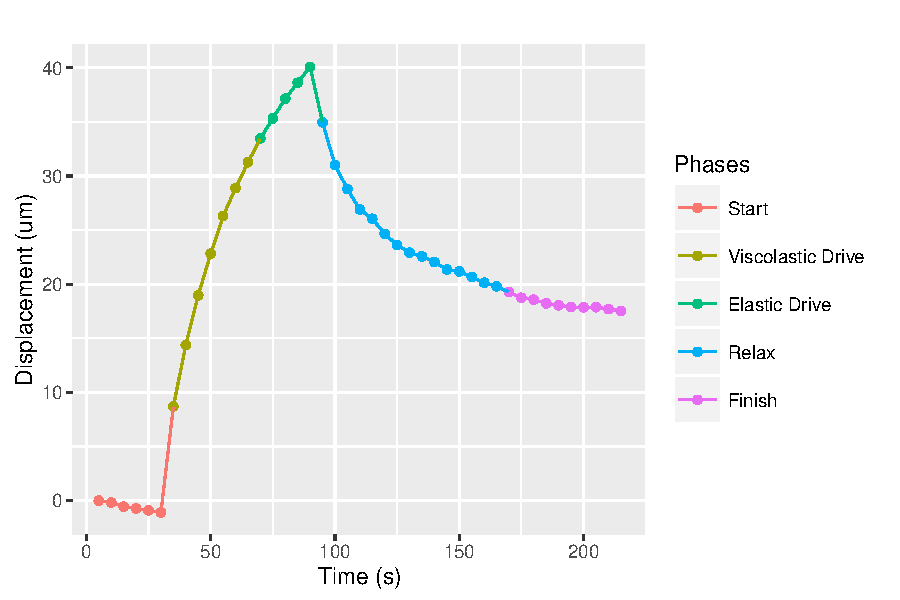
\includegraphics{Chapters/tweezers/Figs/PDF/Displacement_Plot}
%     \caption{Unfiltered reconstruction using a radon transform}
%     \label{fig:}
%   \end{subfigure}\hfill
%   \begin{subfigure}[t]{1\linewidth}
%     \centering
%     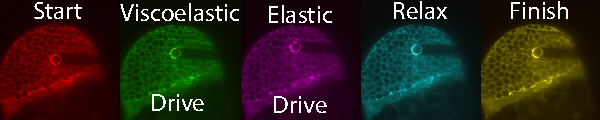
\includegraphics{Chapters/tweezers/Figs/PDF/coloured_fish_stages}
%     \caption{Snapshots in time of each of the stages of drive and recovery.}
%     \label{fig:filtered_recon_helix}
%   \end{subfigure}
%     \hfill
%     \label{fig:flopts}
%   \caption{Comparison of the two reconstructions under sample imaging with a systematic drift, in 3D though represented here in 2D.}
 %\end{figure}

 \begin{figure}
   \centering
    \hfill
       \begin{subfigure}[t]{1\linewidth}
         \centering
         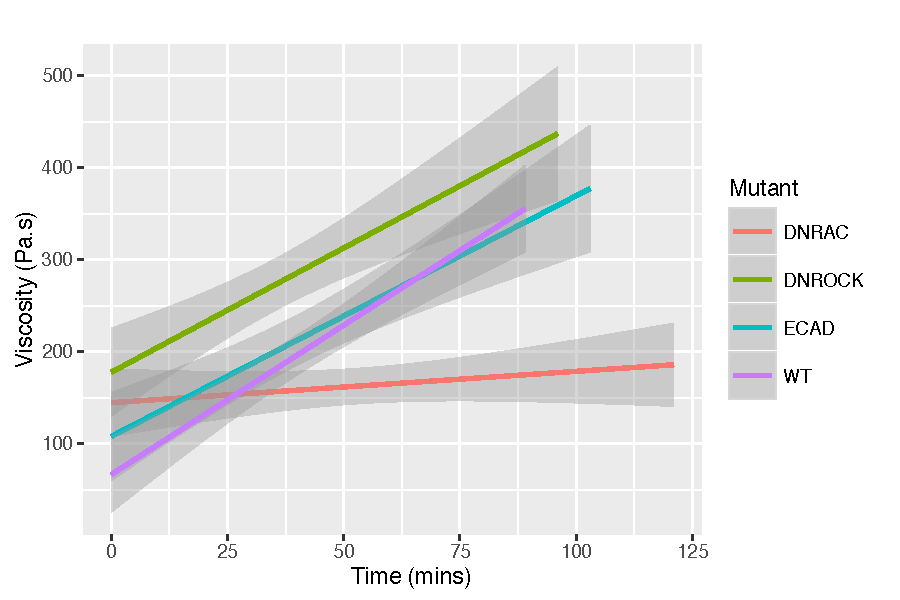
\includegraphics{Chapters/tweezers/Figs/PDF/Cells_-_Time}
         \caption{Change of cellular viscosity $\eta_1$, over time}
         \label{fig:cells_time}
       \end{subfigure}\hfill
          \begin{subfigure}[t]{1\linewidth}
              \centering
              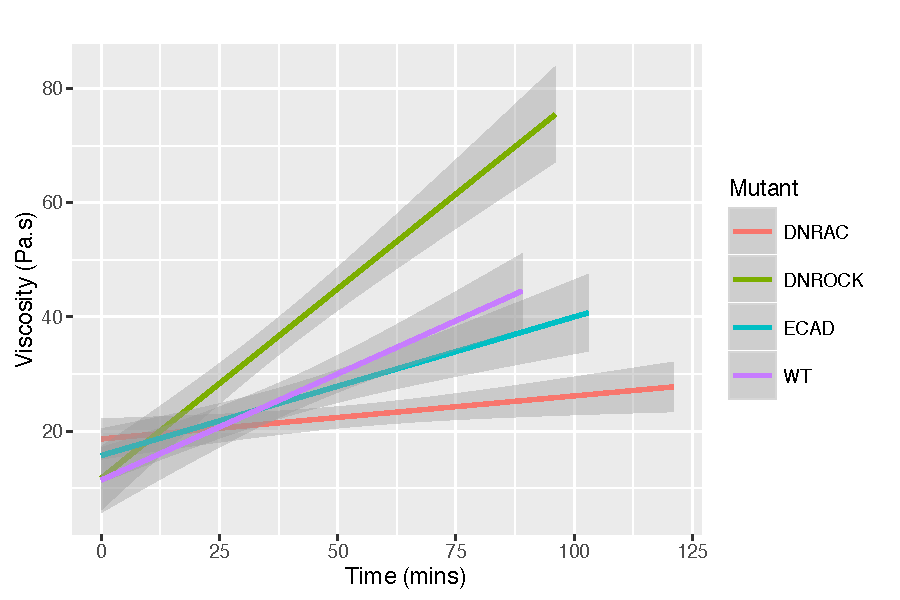
\includegraphics{Chapters/tweezers/Figs/PDF/Tissue_-_Time}
              \caption{Change of tissue viscoity $\eta_2$ over time}
              \label{fig:tissue_time}
          \end{subfigure}\hfill
\end{figure}
\begin{figure}\ContinuedFloat

         \begin{subfigure}[t]{1\linewidth}
           \centering
           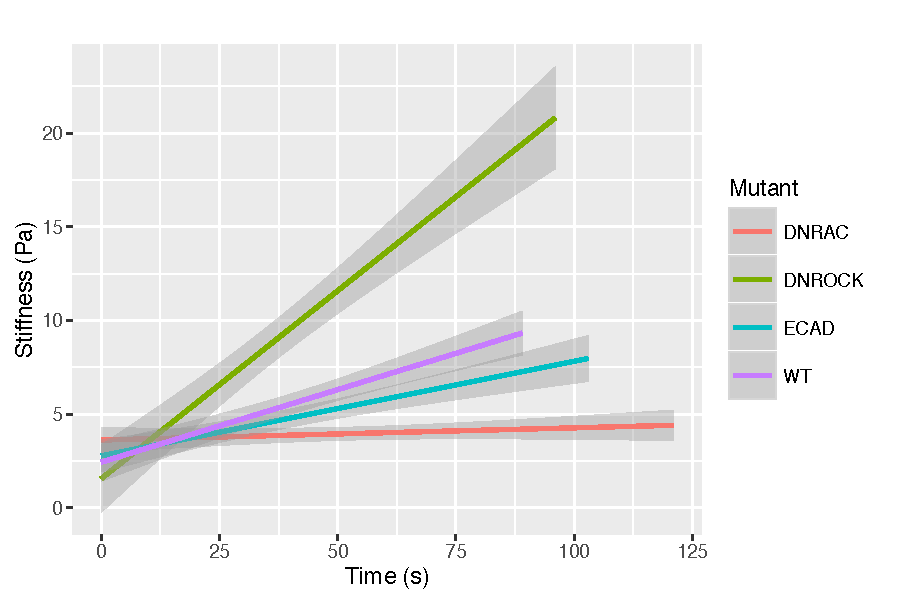
\includegraphics{Chapters/tweezers/Figs/PDF/Stiffness_-_Time}
           \caption{Change of elastic modulus $E$, over time}
           \label{fig:stiffness_time}
       \end{subfigure}\hfill
       \caption{These knock downs have consequences on the developmental evolution of rheological parameters, viscosity coefficients $\eta_1$ \ref{fig:cells_time} and $\eta_2$ (\ref{fig:tissue_time}), and, elastic modulus E (\ref{fig:stiffness_time}): they are decreased in MoECad (n=151 pulls, 9 embryos), and DNRAC (n=158 pulls, 9 embryos) while they are increased in DNROCK (n=107 pulls, 9 embryos) compared to WT (n=178 pulls, 9 embryos).
       \label{fig:visco_time}
       }
\end{figure}

\subsection{Elasticity is linked with cell shape deformation and Viscosity with cell rearrangement.}

To examine how cells around a bead respond during force application, we combined fast light sheet imaging with magnetic tweezers to be enable us to simultaneously track cell shapes and positions during mechanical probing (Figure 3.A-B).
We partition the time course into five periods, based upon the experimental protocol and mechanical signature described above.
We look for cellular correlates of bead displacement in the phases labelled elastic, creep and recoil.
The elastic phase is defined as 3-times the viscoelastic time constant $\tau$ (spanning 95pc of the elastic duration).
The remaining period of active bead displacement is defined as the creep phase (Figure 2.B).
Thirdly, a 3-$\tau$ period of elastic recoil is analysed as the recoil period.
Cell outlines and positions were automatically tracked and manually corrected.
Cell shape changes and cell displacements are measured along the axis of force application to the bead.
Four sectors are defined around the bead relative to this axis (Figure 3.A); we have analysed the front and rear sectors.
As a first approximation, to assess how tissue is elastically-deformed in space, we use an elastic medium force point formula (ref) that couples cell displacement inversely to distance from the centre of force application (the bead), and for a cell shape change stain rate, we use the derivative of this formula.
In front of the bead, during the elastic period, cells are both compressed and displaced forward by its movement (Figure 3.C,D).
This tendency of cells to deform diminishes over development time (Figure 3.F, plinear-regression = 0.016).
In fact, cell shape strain rates are highly correlated with and largely accounts for tissue deformation strain rate (Figure 3F, pcorrelation = 0.0001757, correlation = 0.743).
Cell shape strain rate coefficient is correlated with E (Figure 3.I, pcorrelation = 0.0449, correlation = -0.453).
Behind the bead, we can see a complementary pattern of cell and tissue stretching (Figure S4, correlation = 0.473, p = 0.0748), at all except the earliest developmental stages.
This may be due to incomplete cell adhesion, creating holes in the tissue when the bead moves with excess force.
(In these cases, cell shape change strain rates are not correlated with tissue deformation strain rate.)
When the current is turned off, the shape of cells previous compressed ahead of the bead re-expand back along the force axis (Figure 3.D,H).
Likewise, previously stretched cells behind the bead contract as the bead recoils backwards (Figure 3.D and Figure S4).
We find a good correlation between E and the rate of expansive cell shape deformation in front of the bead (Figure 3.K, correlation = 0.53, p = 0.016).
This is consistent with the rapid elastic bead recoil being determined by an elastic recoil in cell shape, after the release of the imposed force.
We conclude that the cellular signature, of the elastic periods are largely accounted for by cell shape deformations.

\begin{landscape}
  \begin{figure}
    \centering
     \includegraphics[width=\linewidth]{Chapters/tweezers/Figs/PDF/cell_tracking}
      \caption{A-B: Sketch of typical rheological experiment (A) in WT embryo under SPIM (B) where blue represents cell extension and red is compression. 1-2-3 label regarding cells over time-lapse.
      Yellow dot marks the original position of the bead centre.
      C-D: Analysis of the coefficient of deformations $C_t$ and $C_C$ shows that tissue (C) and cells (D) are compressed at the front of the bead while they are stretched are the rear during bead pulling (n = 14 pulls, 3 embryos).
      E-H: Analysis of cell area and cell aspect ratio reveals cells disappear from imaging plane, suggesting cells at the front rearrange in 3D, while at rear, cells are stretched (E).
      Along developmental time, tissue deformation ($C_t$), cells deformation ($C_c$) and cell intercalation ($C_t$-$C-s$) during elastic phase (in \SI{}{\micro\metre\squared\per\minute}), at the front of the bead, show that tissue compression can be accounted mainly by cell shape changes (F), while, during creep phase, strain rates show that this accountancy is lost, suggesting cell rearrangement is major event (G).
      When force is released, cells at the front relax to their original shape (H).
      I-K: Correlation analysis of cell parameters and rheological parameters.
      This is supported by correlations between elastic modulus E and cell shape change coefficient during elastic phase, at the front of the bead (I), between viscosity coefficient $\eta_1$ and cell rearrangement rate during creep phase (J), between elastic modulus $E$ and cell shape change coefficient during recoil phase (K).
      Lines represent linear regressions.
      }
      \label{fig:cell_tracking}
  \end{figure}
\end{landscape}

To investigate how tissue deforms during the creep phase, which in the mechanical model is defined by $\nu$1, we visually inspected how cells in tissue in front and behind the bead behaved during this period.
We see cells becoming compressed and moving out the plane (decreasing in area), in front of the bead and conversely cells becoming stretched and entering the plane at the rear (Figure 3 A, B).
This behaviour can be quantified by comparing changes in cell aspect ratio and area through both the elastic and creep periods (Figure 3.E).
Early cell shape changes give way to area changes during the creep period, which we interpret as the result of cells rearranging in the tissue in front and behind the bead.

To quantify cell behaviours during the creep period, we measure cell and tissue strain rates using a simplified tissue tectonics approach (REF).
Tissue strain rate, cell shape strain rate and cell rearrangement rates are measured along the direction of force application (see M\&M).
While the elastic periods were dominated by changes in cell shape, the creep period is characterised by cell rearrangements.
Cell shape strain accounts for a small fraction of tissue strain rate (Figure 3.G), and does not correlate with $\nu$1 (front correlation = 0.345, p = 0.21; rear correlation = -0.052, p = 0.85).
Nonetheless, measureable cell shape strain rates indicate some contribution persists through the creep period.
However, cell intercalation strain rate does correlate with $\nu$1, both in front (Figure 3.J, pcorrelation = 0.0638, correlation factor = 0.49) and behind the bead (Figure S4, p = 0.035, correlation = -0.546).
We conclude that cell rearrangements are the major determinants of tissue viscosity in the creep period.

%Good \/

\subsection{Modifications of cell motility and migration lead to defects in early embryogenesis and tissue rheology.}

The results of analysing %cell shape changes and
movement during bead displacement are consistent with our simple hypothesis of a two-component model.
%To test this hypothesis further, we have manipulated embryos to modulate their cellular properties.
We will measure how these changes affect embryo development, %cell behaviours
and the mechanical properties of the blastoderm.
Cell adhesion is a fundamental requirement for building a cohesive tissue, we reduced expression of E-Cadherin (cdh1).
Using a knock-down Morpholino approach (MoECad), we show that knockdown of cell adhesion leads to embryos defective in the high-to-sphere transformation; these embryos failed to achieve a spherical shape (Figure 4.A).
%At a cellular level, cell protrusions lose their radial polarity (Figure S5), while the number of protrusion per cell are not different (Figure 4B, C).
%Further, cells in treated embryos have a reduced coefficient of diffusion (6.3 µm2/min, pWT-MoECad = 1.6*10-5), showing them less able to migrate as extensively as WT cells (Figure 4.B, p = 1.621e-05), though the directions of migration are as seen in WT ****[Check those directions].
Rheological measurements show that MoECad-treated embryos remain less stiff and less viscous than their WT counterparts.
Further, they are reduced in the elevation of these properties over developmental time \ref{fig:visco_time}
Developmental trends are significantly different to WT, $p_E = 5.63e-07$ , $p_{\nu_1} = 2.10e-03$, $p_{\nu_2} =0.042$).

We have identified that cell migration and cell protrusive activity are two major cell behaviours at these stages.
Small GTPases are identified as central orchestrators of cell polarity and motility %TOOD cite 23.
Two complementary molecular components of cell migration, Rac1 signalling were manipulated,
Rac1 signalling using a dominant-negative Rac1 construct (DNRAC, ref), RhoA signalling by a dominant-negative Rho-kinase construct (DNROCK, %TOOD cite 24
).
DNRAC we anticipate should eliminate protrusive activity, while DNROCK would reduce the activation of the molecular motor myosin-2.
The injection of these dominant negative constructs affect early morphogenesis, DNRAC-injected embryos fail to progress to a spherical shape, while DNROCK injection causes a faster round-up of the embryo.
%Myosin-2 inhibition via blebbistatin treatment gives the same phenotype as DNROCK treatment (Figure S5).
%At a cellular level, cells in DNRAC-injected embryos produce far fewer protrusions (Figure 4B, freqWT = 2.05 extensions/frame/cell, freqDNRAC = 0.4 extension/frame/cell, p = 0.01386).
%Cells in DNROCK-injected embryos make significantly more protrusions than WT (Figure 4B, freqDNROCK = 5.30 extensions/frame/cell, p = 0.0007866) and more cells display a multipolarity (Figure 4.C).
%Cell protrusions in DNROCK-injected embryos favour a radial distribution but are more dispersed and numerous than WT (Figure S6).
%The increase in protrusion production in DNROCK embryos is as expected for a loss of function of myosin-2 in migratory cells [ref].
%(Protrusions on DNRAC injected cells are too infrequent to perform statistical analyses.)
%Within DNRAC-injected embryos, the apparent diffusion of cells is significantly reduced compared with WT (4.3 µm2/min, pWT-DNRAC = 10-8).
%Apparent cell diffusion in DNROCK-injected embryos is significantly increased compared with WT (29.9 µm2/min, pWT-DNROCK = 0.000433).
%**** Analyses of cell migration directions in DNRAC are …., and in DNROCK appears as in WT (Figure S6).
%In addition, recruitment of myosin-2 to the cell cortex is greatly reduced in DNROCK-treated cells (Figure S7).
%Cortical myosin2 resembles the WT distribution in both DNRAC and MoECad injected embryos (Figure S7).
%Interestingly, at both cellular and embryonic levels, the phenotypes of DNRAC and DNROCK treated embryos differ from WT in opposite ways, including embryo morphology, cell protrusion formation, cell migration and cell dispersion.
%In the light of the MoECad results, we would predict that the physical properties of DNRAC-injected embryos should be less stiff and less viscous than WT those for DNROCK-injected would be stiffer and more viscous.
When we measure those rheological parameters by magnetic bead displacement, we confirm these predictions: DNRAC embryos fail to increase stiffness and viscosities $\nu$1 and $\nu$2 (pE = 1.016e-09, p$\nu$1 = 1.87e-04, p$\nu$2 = 0.0028) while DNROCK embryos become stiffer and more viscous (pE = 7.59e-25, p$\nu$1 = 6.74e-15, p$\nu$2 =3.65e-12) than their WT counterparts (Figure 4.F-H).
Interestingly, $\tau$ is affected by the different knock downs, stiffer embryo showing a shorter $\tau$ than softer ones (all p << 1e-5).

Finally, we wished to ask how the changes rheological properties found for DNRAC and DNROCK treatments are reflected in the rates of cell and tissue deformation?
We repeated fast light sheet imaging analyses with each knock-down treatment, to follow cell behaviours during force application.
The resultant parameters do segregate according to their mechanical properties: softer DNRAC embryos present more cell deformation during the elastic period ($p_{WT-DNRAC} = 0.0013$) and more cell rearrangement during the creep period ($p_{WT-DNRAC} = 0.0025$), compared to WT.
Cells in the stiffer DNROCK-injected embryos deform less in the elastic period ($p_{WT-DNROCK} = 0.0017$) and induce less cell rearrangement in the creep period ($p_{WT-DNROCK} = 0.0013$) %TODO figure (Figure 4.J).
%We can now combine data from all WT and experimental manipulation conditions to examine correlations within an extended range of developmental conditions.
These results confirm the previously-observed correlations between cellular and rheological parameters hold true under this expanded range.
Stiffness E is strongly correlated with initial cell shape deformation while $\nu$1 is strongly correlated with cell rearrangements.
This suggests that there may be a relatively simple cellular interpretation of the physical model measured using magnetic bead rheology.
Since the measurement of bead movements are faster, easier and more sensitive than the associated cell measurements, this facilitate us gaining greater insight into the mechanics of developing tissues.

\subsection{Biological methodology}
Embryos were harvested just after fertilisation and incubated at 28.5ºC.
Used lines were: wild types (WT), Tg(beta-actin:mCherry-CAAX) (labelling membranes), Tg(beta-actin:Lifeact-eGFP) (labelling F-actin) and Tg(beta-actin:Myosin2-mCherry).

\subsubsection{Bead and cell transplantation}
Transplantations were at 1k-cell stage using a tip broken elongated capillary (REF) mounted on an oil filled pressurised system controlled by a syringe (REF).
Beads or cells were transplanted at 1k-cell stage.
The Superparamagetic beads used in this work are polystyrene spheres filled with nanoparticles of iron oxide and are 41.14 µm diameter.
Beads were incubated in 4\% BSA before grafting to reduce chances of bead rejection when injected.

\section{Discussion}
%New technique for remote measurement of biological forces
In this study, we have shown for the first time the direct link between cell behaviours and embryo morphogenesis through their measured mechanical properties, in the of the zebrafish blastula simple morphogenetic transformation. %TODO check this line
We could apply directed force within a tissue and challenge this tissue mechanically and report the response of the tissue at cellular level.
We also showed that these properties are controlled at molecular level, through a network made of actomyosin and cadherin as knock downs of Rac1, Rho-kinase and E-Cadherin have dramatic repercussions on all levels, from cell to embryo.


\subsubsection{Rear versus Front}
It is still not clear what happens at the rear of the bead, especially at early stages.
The bead is not coated with any molecules.
The way the bead is contacting surrounding cells is thus dependent on how cells are adhesive between each other.
When this adhesion is weak, at early stages in WT, or in soft embryos, gaps are observed at the rear.
Doing so, the cells are not pulled by the bead movement.
When the connectivity becomes stronger, we can clearly a stretch of the cells at the rear that is proportional to E.

\subsubsection{Recovery phase}
After ~45sec sec after cutting the current off, the rheological model lack to explain the bead movement.
What could possibly happen is that we enter a phase during which morphogenetic movement is overtaking bead movement as cells are active.

\subsubsection{Is myosin-2 activity acting unexpectedly?}
Inhibition of cell contractility gives at rheological level unexpected results: absence of myosin-2 activity gives rise to stiffer embryo.
Canonically, myosin controls cell contractility and loss of contractility leads to softer cell cortex.
Nonetheless, these expectations are mostly rising from epithelium and single cell studies.
Here, the tissue is strictly mesenchymal and cells present a strong protrusive activity.
In fact, at cellular levels, it is known that regulation of actomyosin mechanics is dependent on the nature of the cell, as well as how cells are organised.
For instance, myosin-2 is controlling cell cortex stiffness, but in two different ways: for cells in suspension, myosin-2 softens the cortex, while, if cells are plated on a dish, myosin-2 stiffens it.
This paradox behaviour is also noticed at molecular levels, when myosin activity can soften or stiffen the actin network, regarding what molecular actors are present.
Expectations about myosin incidence on cell and tissue stiffness must take in account the cell organisation and how cells connect to each other.

\subsubsection{Connectivity: rising of tissue properties}
Interestingly, we demonstrate that the emergence of mechanical properties is linked with the motility of the cell.
In particular, we showed that dynamics of protrusive activity and cell-cell adhesion are two main actors.
This suggests that the establishment of connection between the cells is a key factor and control of coherent tissue.
This connectivity can be seen as a superstructure of the actomyosin network connected between cells through cell adhesion molecules, such as E-Cadherin.
This network would be dependent upon how cells contact each other through cell extensions, a turnover between stable contacts and new contacts, and, upon how this network grows and contract.
[Maybe do here a hypothesis about syntitial embryos of Drosophila]

\subsubsection{Correlation of rheological parameters}
Intriguingly, we were not able to uncouple the different mechanical parameters in the three different knockdowns we looked at.
Parameters variate in the same direction.
It is still unclear the fundamental mechanisms by which a particular type of molecules could influence all parameters.
This suggests strongly that tissue rheology is regulated at higher level than simply molecular and cellular.
It shows that even if cells and molecular network have their own mechanical specificities, they must be integrated in a greater framework to predict their properties.

\subsubsection{analysis}
All tests were performed with R software.
Student's t-test were performed for ellipse ratio and mean square displacement analyses. %Probably not including?
Linear mixed effect model was performed to compare rheological parameter trends in different loss-of-function essays.
Anova test compared linear fits on developmental trends of the rheological parameters between WT and loss of function conditions.
Percentage bend correlation method was used for correlation between cell and rheological parameters, to take in account outliers.
